\subsection{Vacuum Cleaner (Toy problem) \cite{ai/book/Artificial-Intelligence-A-Modern-Approach/Russell-Norvig}}


\begin{figure}[H]
    \centering
    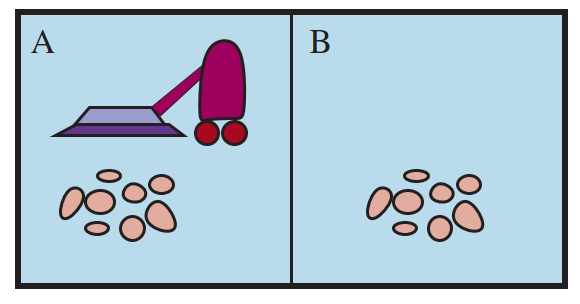
\includegraphics[
        width=0.5\linewidth,
        height=3cm,
        keepaspectratio
    ]{images/artificial-intelligence/examples/vacuum-cleaner-world.png}
    \caption*{A vacuum-cleaner world with just two locations}
\end{figure}

\begin{figure}[H]
    \centering
    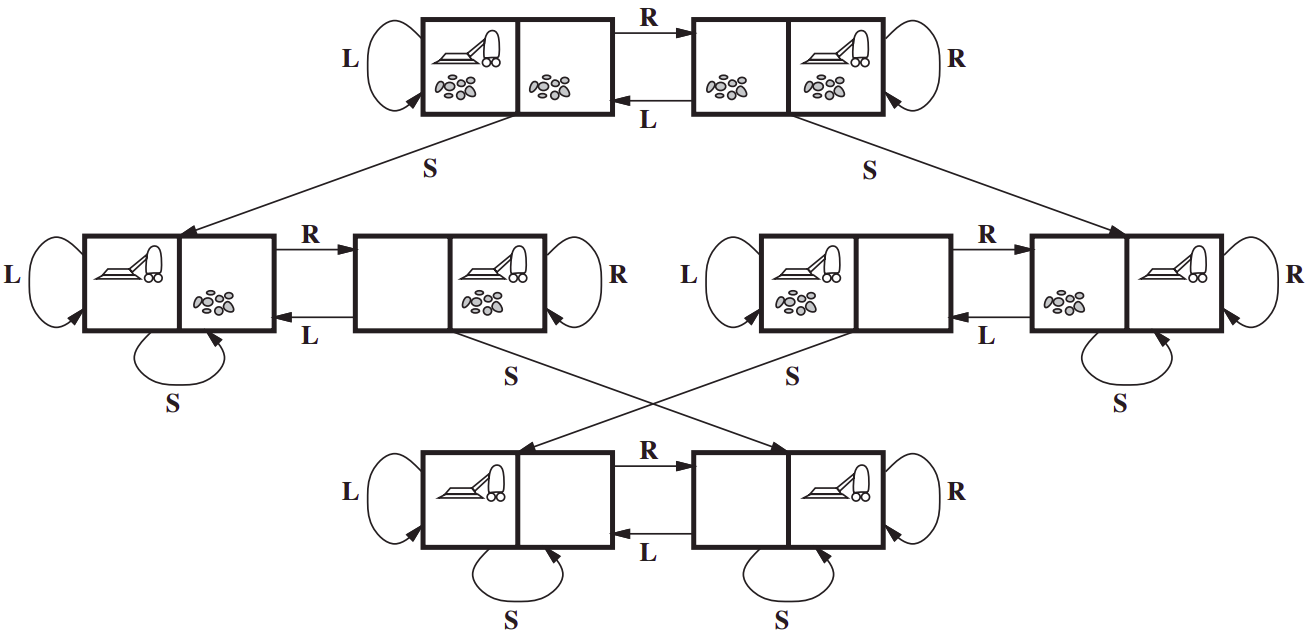
\includegraphics[
        width=\linewidth,
        % height=7cm,
        keepaspectratio
    ]{images/artificial-intelligence/examples/vacuum-state-space.png}
    \caption*{The state space for the vacuum world. Links denote actions: L = Left, R = Right, S= Suck. \cite{ai/book/Artificial-Intelligence-A-Modern-Approach/Russell-Norvig}}
\end{figure}



\vspace{0.5cm}

\begin{enumerate}[itemsep=0.2cm]
    \item it’s a made-up world

    \item This particular world has just two locations: squares A and B. 
    
    \item The vacuum agent perceives which square it is in and whether there is dirt in the square. 
    
    \item It can choose to \textbf{move left}, \textbf{move right}, \textbf{suck up the dirt}, or \textbf{do nothing}.

    \item One very simple agent function is the following: if the current square is dirty, then suck; otherwise, move to the other square.

    
\end{enumerate}



\subsubsection{As a table driven agent}

\begin{customArrayStretch}{1.3}
\begin{longtable}{|l|l|}

\hline
\textbf{Percept sequence} & \textbf{Action} \\ \hline
\endhead

\hline
\textbf{Percept sequence} & \textbf{Action} \\ \hline
\endfirsthead

\hline\endfoot
\hline\endlastfoot


$[A, \ Clean]$ & $Right$ \\ 
$[A, \ Dirty]$ & $Suck$ \\ 
$[B, \ Clean]$ & $Left$ \\ 
$[B, \ Dirty]$ & $Suck$ \\ 

\vdots & \vdots \\

$[A, \ Clean],\ [A, \ Clean]$ & $Right$ \\ 
$[A, \ Clean],\ [A, \ Dirty]$ & $Suck$ \\ 

\vdots & \vdots \\

$[A, \ Clean],\ [A, \ Clean],\ [A, \ Clean]$ & $Right$ \\ 
$[A, \ Clean],\ [A, \ Clean],\ [A, \ Dirty]$ & $Suck$ \\ 

\vdots & \vdots \\

\end{longtable}
\end{customArrayStretch}





\subsubsection{As a simple reflex agent}

\begin{algorithm}[H]
    \caption{The agent program for a simple reflex agent in the two-state vacuum environment.  \cite{ai/book/Artificial-Intelligence-A-Modern-Approach/Russell-Norvig}}

    \SetKwFunction{FUNCTION}{\textsc{Reflex-Vacuum-Agent}}
    \SetKwProg{Fn}{function}{ returns \normalfont{an action}}{end}
    \Fn{\FUNCTION{[location, status]}}{
        \textbf{if} $status \ = \ Dirty$ \textbf{then return} $Suck$ \\

        \textbf{else if} $location \ = \ A$ \textbf{then return} $Right$ \\

        \textbf{else if} $location \ = \ B$ \textbf{then return} $Left$ \\
    }
\end{algorithm}







\subsubsection{As a problem solving agent}

\begin{enumerate}[itemsep=0.2cm]
    \item \textbf{States}: The state is determined by both the agent location and the dirt locations. The agent is in one of two locations, each of which might or might not contain dirt. Thus, there are $2 \times 2^2\ =\ 8$ possible world states. A larger environment with $n$ locations has $n \cdot 2^n$ states.

    \item \textbf{Initial state}: Any state can be designated as the initial state.

    \item \textbf{Actions}: In this simple environment, each state has just three actions: Left, Right, and Suck. Larger environments might also include Up and Down.

    \item \textbf{Transition model}: The actions have their expected effects, except that moving Left in the leftmost square, moving Right in the rightmost square, and Sucking in a clean square have no effect.

    \item \textbf{Goal test}: This checks whether all the squares are clean.

    \item \textbf{Path cost}: Each step costs $1$, so the path cost is the number of steps in the path.
\end{enumerate}











